%%%%%%%%%%%%%%%Conjectures regarding values of Riemann zeta function at Gram points%%%%%%%%%%%%%%%%%%%%%%%%%%%%%%%%%%%%%%%%%%%%%%%%%%%%%%%%%%%%%
%

\documentclass[twoside]{article}
\usepackage{graphicx}
\usepackage{amsmath,amsthm,amssymb,verbatim}
\usepackage{fancyhdr}
\pagestyle{fancy}
\usepackage{url}
\usepackage{xcolor}


\def\blfootnote{\xdef\@thefnmark{}\@footnotetext} 
\long\def\symbolfootnote[#1]#2{\begingroup%
\def\thefootnote{\fnsymbol{footnote}}\footnote[#1]{#2}\endgroup} 

\newtheorem{mydef}{Conjecture}
\newtheorem*{mydef-non}{Conjecture}

\theoremstyle{definition}
\newtheorem{defn}{Definition}

\setcounter{page}{1}
\begin{document}

\date{}
\lhead[]{}
\chead[]{}
\rhead[]{}

\title{\bf{Symmetry properties of distribution of Riemann Zeta Function values on critical axis}}
%

\author{O. Shanker 
 \thanks{Mountain View, CA 94041, U. S. A. Email: oshanker@gmail.com
 }
}

\maketitle
\thispagestyle{fancy}

\begin{abstract}
Symmetry properties  of the Riemann Zeta Function are important, because the celebrated Riemann Hypothesis has so far
resisted all attempts at a proof or disproof. Symmetry properties can provide guidelines to attacking the problem. The symmetry
properties are also interesting in themselves. In this work we study new conjectured symmetry properties for the distribution
of zeta function values on the critical axis.
\end{abstract}

\symbolfootnote[0]{
\url{https://sites.google.com/site/riemannzetazeros/conjectures} 
}


%\clearpage
\chead[\underline{O. Shanker}]{\underline{Symmetry properties of distribution of Riemann Zeta Function values on critical axis}}


\section{Introduction}
In this work we discuss the symmetry properties of the distribution of Riemann zeta values on the critical axis. 
Understanding such symmetry properties is important, because the celebrated Riemann Hypothesis has so far
resisted all attempts at a proof or disproof. The study of the symmetry properties  will give us insight into the theoretical underpinnings of the location of zeros of the Riemann Zeta Function.
The new results are stated in Equations \ref{eq:mean}, \ref{eq:antisym} and \ref{eq:sym} (Section~\ref{conjectures}), after we set up the
required notation (see Section~\ref{sec2}). These results are a generalization of the result in Ref.~\cite{Shanker 2018} for the anti-symmetry of the distribution of $Z(t)$ at even and odd Gram points. 

The paper is organized as follows.
Section~\ref{sec2} establishes the required notation for the 
Riemann Zeta Function and presents the conjectured symmetry relations. 
Section~\ref{sec3} provides evidence for the symmetry relations.
Section~\ref{conclusions} presents the conclusions.

\section{\label{sec2}Notation for the Riemann zeta function and the symmetry properties}

In this section we  establish the required notation for the 
Riemann Zeta Function. We follow closely the treatment in Ref.~\cite{Shanker 2018}.
For $\mathrm{Re} (s) > 1$ the Riemann Zeta function is defined as
\begin{equation}
\zeta ( s ) \, = \, \sum^{\infty}_{n = 1} \; n^{-s} \, = \, \prod_{p \in primes} \;
\left( 1 - p^{-s} \right)^{-1}.
\label{eqRie}
\end{equation}
 $\zeta ( s )$ can be continued to
the complex plane. It satisfies the functional equation \cite{Riemann(1858),Riemann 1892, Titchmarsh 1986,Edwards(1974)}
\begin{equation}  
\xi(s):=s(s-1) \pi^{-s/2} \, \Gamma (s/2) \, \zeta ( s )/2 \, = \, \xi ( 1 - s );
\label{eq:xifunc}
\end{equation}
$\xi(s)$ is an entire function. The zeroes of $\xi(s)$ are denoted by $1/2 + i \gamma$. The Riemann Hypothesis  
is that $\gamma$ is real for the non-trivial zeroes.
The $\gamma$s are ordered in increasing order, with 
\begin{equation}
\ldots \ldots \gamma_{-1} \, < \, 0 \, < \, 
\gamma_1 \, \leq \, \gamma_2 \ldots. 
\end{equation}
Then $\gamma_j \, = \, - \gamma_{-j}$ for $j = 1, 2, \ldots,$ 
and    $\gamma_1$, $\gamma_2$, $\ldots$  are roughly
$14.1347$, $21.0220$, $\ldots$. The line $1/2 + it$ is called the critical axis.

Asymptotically, the mean number of 
zeros for the Riemann zeta function with height less than $t$ (the smoothed Riemann zeta staircase, denoted by 
$N_{smooth}(t)$) is~\cite{Edwards(1974)}
\begin{equation}  
N_{smooth}(t) = (t/2\pi)(\ln(t/2\pi)-1)+\frac{7}{8}.
\label{eq:Rnumber}
\end{equation}
Thus, the mean spacing $\delta$ of the zeros at height $t$ is 
\begin{equation}  
\delta = 2\pi(\ln (t/2\pi))^{-1}. 
\label{eq:spacing}
\end{equation}
One defines
\begin{equation}
\theta(t) = arg (\pi^{it/2} \Gamma(\frac{1}{4} + \frac{it}{2})), 
\label{eq:theta}
\end{equation}
where the argument is defined by continuous variation of $t$ starting with the value $0$ at $t = 0$.
For large $t$, $\theta$ has the asymptotic expansion
\begin{equation}
\theta(t) \approx \frac{t}{2}\ln (\frac{t}{2\pi}) - \frac{t}{2} - \frac{\pi}{8} + \frac{1}{48t} - \frac{1}{5760t^3}. 
\label{eq:thetaAsymptotic}
\end{equation}
From the zeta functional equation it follows that Hardy's function 
\begin{equation}
Z(t)=exp(i\theta(t))\zeta(1/2 +it) 
\label{eq:hardy}
\end{equation}
is real valued for real $t$. 
Moreover we have $|Z(t)| = |\zeta(1/2+it)|$. Thus the zeros of $Z(t)$ are the imaginary part of the zeros 
of $\zeta(s)$ which lie on the critical line.  

Many of the zeros are separated by the
Gram points~\cite{Gram 1903}.  When $t \ge 7$, the $\theta$ function Eq.(\ref{eq:theta}) is monotonic increasing. 
\begin{defn}\label{gram}
For $n \ge -1$, the $n$-th Gram point $g_n$ is defined as the unique solution $> 7$ to
$\theta (g_n) = n\pi$. We call the Gram point an odd Gram point if $n$ is odd, and an even Gram point if $n$ is even.
A Gram interval is the interval $G_n = [g_n,g_{n+1})$.
\end{defn}
Thus, at a Gram point we have
\begin{equation}
\zeta(1/2+ig_n) = (-1)^{n}Z(g_n).
\label{eq:zetagram}
\end{equation}
Ref.~\cite{Shanker 2018} studied empirically the distribution of $Z(t)$ values at Gram points. We will generalize the study to other points on
the critical axis, as defined below. In analogy with Gram points, we can associate an angle $\phi$ with a point $t$ on the critical axis as follows:
\begin{defn}\label{phi}
For $t \ge 7$, $t$ is said to be a phi point if
$\theta (t) = 2k\pi + \phi$, where $0 \le \phi < 2\pi$.
\end{defn}
An odd Gram point has $\phi=\pi$ and an even Gram point has $\phi = 0$. We will study the distribution of $Z(t)$ values at a given value of $\phi$, and investigate symmetry and anti-symmetry relations for the 
distributions at different values of $\phi$. Formally, our sample space is defined by
\begin{defn}\label{samplespace}The sample space for all the distributions in this work is an interval  at height $t$ which is large compared to the Gram interval, but small enough that  we can divide the sample space into a small number of sub-intervals, where $\ln (t)$ can be considered to be effectively constant over each sub-interval. 
\end{defn}
The latter condition is not essential but is convenient, in that it simplifies the numerical work. We divide our sample space into $34$ sub-intervals, and we take $\ln (t)$ to be  constant over each sub-interval.
The notation $\ln (t)$ stands for the natural logarithm of $t$.  We define $p_{\phi}(y)$, the probability distribution function for $Z(t)$ at phi points:
\begin{defn}\label{pphi}
\begin{equation}
\int\limits_{a}^{b} p_{\phi}(y)dy
\label{eq:pdfphi}
\end{equation}
is the probability that $a<Z(t)<b$ when we consider the values of $Z(t)$ for a large number of phi points in the sample space. 
\end{defn}
In Ref.~\cite{Shanker 2018}  we defined $p_{odd}(y)$ as
\begin{defn}\label{podd}
\begin{equation}
\int\limits_{a}^{b} p_{odd}(y)dy
\label{eq:pdfodd}
\end{equation}
is the probability that $a<Z(t)<b$ when we consider the values of $Z(t)$ for a large number of odd Gram points in the sample space. 
\end{defn}
$p_{even}(y)$ was defined analogously. In terms of Definition~\ref{pphi} we have $p_{odd}(y) = p_{\pi}(y)$ and $p_{even}(y) = p_{0}(y)$.
The probability densities $p_{odd}(y)$,  $p_{\phi}(y)$ and $p_{even}(y)$ depend on the sample space (i.e., on the height $t$ and on the size of the sample space). In practice the densities are not sensitive to the choice of the sample space as long as the height $t$ is large enough and the length of the interval from which the sample is collected is large enough (but not too large on log scale).

\subsection{\label{conjectures}Conjectures}

Ref.~\cite{Shanker 2018} conjectured that $p_{odd}(y) = p_{even}(-y)$. We generalize the conjecture as stated in Equations \ref{eq:mean}, \ref{eq:antisym} and \ref{eq:sym} below.
Our first new conjecture is that the mean value $\langle Z(t_{\phi})\rangle$ is given by
\begin{equation}
\langle Z(t_{\phi})\rangle = 2\cos (\phi).
\label{eq:mean}
\end{equation}
Equation \ref{eq:mean} was explicitly called out for Gram points ($\phi = 0$ and $\phi = \pi$) in Ref.~\cite{Titchmarsh 1934}. The proof of Ref.~\cite{Titchmarsh 1934} can be extended to cover Equation \ref{eq:mean}. Our other two conjectures are that $p_{\phi}(y)$ satisfies the anti-symmetry condition
\begin{equation}
p_{\phi}(y) = p_{\phi+\pi}(-y),
\label{eq:antisym}
\end{equation}
and the symmetry condition
\begin{equation}
p_{\phi}(y) = p_{2\pi-\phi}(y).
\label{eq:sym}
\end{equation}
The empirical evidence for these generalizations is given in the next section.

\section{\label{sec3}Evidence for the symmetry relations}

For the empirical validation of the mean value condition  Equation \ref{eq:mean}, the anti-symmetry condition  Equation \ref{eq:antisym} and the symmetry condition  Equation \ref{eq:sym} we have to evaluate $Z(t)$ at several points on the critical axis. We chose our sample space to
be $10^6$ Gram intervals starting at $t=10^{12} + 243.777560$ (which is a Gram point with Gram index $3945951431271$). We chose this sample space because  Ref~\cite{hiary 2010} has evaluated all the zeros in this range. We used the  zeros from Ref~\cite{hiary 2010} to check the accuracy of our zeta function calculations. Our evaluations of $Z(t)$ are accurate to better than $10^{-6}$.

\subsection{\label{numerics}Numerical evaluation}

Hardy's function $Z(t)$  is evaluated using the Riemann$-$Siegel series
\begin{equation}
Z(t) = 2\sum^{m}_{n=1}\frac{\cos(\theta(t) - t \ln (n))}{\sqrt{n}} + R(t), 
\label{eq:RS}
\end{equation}
where $m$ is the integer part of $\sqrt{t/(2\pi)}$. $R(t)$ is a small remainder
term which can be evaluated to the desired level of accuracy. We used the techniques in Refs.~\cite{Odlyzko 1992,hiary,gourdon} 
to efficiently evaluate the zeta function at large $t$. The most important 
source for loss of accuracy at large heights is the cancellation between
large numbers that occur in the arguments of the $\cos$ terms in Eq.~(\ref{eq:RS}). We 
use a high precision module to evaluate the arguments. The rest of the calculation
is done using regular double precision accuracy. 

\begin{table}
\centering \(\begin{array}{ccccccc}
\hline
 \phi &     Min.   & 1st    &  Median    &   Mean   & 3rd    &   Max. \\
 &              & Quantile   &            &              & Quantile.    &   \\
\hline
0 &-69 &0.1134 &0.8517 &2.0001 &2.5403 &165  \\
\pi/4 &-97 &-0.1352 &0.5916 &1.4143 &2.1226 &159 \\
\pi/2 &-121 &-1.082 &0.0017 &0.0001 &1.089 &137 \\
3\pi/4&-148 &-2.1121 &-0.5852 &-1.4141 &0.1364 &103 \\
\pi &-161 &-2.5277 &-0.8467 &-1.9999 &-0.1122 &69 \\
5\pi/4 &-153 &-2.1045 &-0.5891 &-1.4141 &0.1365 &105 \\
3\pi/2 &-129 &-1.083 &-0.001 &0.0001 &1.084 &138 \\
7\pi/4 &-93 &-0.1336 &0.5883 &1.4143 &2.1077 &160 \\
\hline
\end{array}\)
\caption{Quantiles and mean for  $Z(t)$ when $\phi$ values are multiples of $\pi/4$.} 
\label{tab:quantiles}
\end{table}

\begin{table}
\centering \(\begin{array}{ccccccc}
\hline
 \phi &     Min.   & 1st    &  Median    &   Mean   & 3rd    &   Max. \\
  &              & Quantile   &            &              & Quantile.    &   \\
\hline
0 & -69 & 0.1134 & 0.8517 & 2.0001 & 2.5403 & 165 \\
\pi/6 & -88 & 0.0167 & 0.7318 & 1.7321 & 2.3515 & 162\\
\pi/3 & -105 & -0.3877 & 0.4108 & 1.0001 & 1.8151 & 154\\
\pi/2 & -121 & -1.082 & 0.0017 & 0.0001 & 1.0888 & 137\\
2\pi/3 & -140 & -1.81 & -0.4053 & -0.9999 & 0.3904 & 115 \\
5\pi/6 & -155 & -2.338 & -0.7258 & -1.732 & -0.0160 & 91\\
\pi & -161 & -2.5277 & -0.8467 & -1.9999 & -0.1122 & 69\\
7\pi/6 & -158 & -2.334 & -0.7294 & -1.732 & -0.0161 & 93\\
4\pi/3 & -147 & -1.8034 & -0.4097 & -0.9999 & 0.388 & 117\\
3\pi/2 & -129 & -1.083 & -0.001 & 0.0001 & 1.0842 & 138\\
5\pi/3 & -105 & -0.3855 & 0.4086 & 1.0001 & 1.8103 & 154\\
11\pi/6 & -80 & 0.0184 & 0.7317 & 1.7322 & 2.3393 & 164 \\
\hline
\end{array}\)
\caption{Quantiles and mean for  $Z(t)$ when $\phi$ values are multiples of $\pi/6$.}
\label{tab:quantiles6}
\end{table}

\subsection{\label{quantiles}Quantiles}
Table~\ref{tab:quantiles} shows the quantiles and mean for  $Z(t)$  when $\phi$ values are multiples of $\pi/4$.  The column showing the mean of the distribution clearly validates the mean value condition Equation~\ref{eq:mean}. The anti-symmetry condition Equation~\ref{eq:antisym} can be checked, for example, by validating that rows 2 and 6 of the table have anti-symmetric distribution parameters (row 2 has $\phi=\pi/4$ while row 6 has $\phi=5\pi/4$). The symmetry condition Equation~\ref{eq:sym} can be checked by verifying, for example, that rows 2 and 8 of the table have the same distribution parameters (row 2 has $\phi=\pi/4$ while row 8 has $\phi=7\pi/4$). The equation also states that rows 4 and 6 of the table have the same distribution parameters (row 4 has $\phi=3\pi/4$ while row 6 has $\phi=5\pi/4$). Repeated application of Equation~\ref{eq:antisym} and Equation~\ref{eq:sym} gives us the relation between the distributions at $\phi$,  $\pi-\phi$,  $\pi+\phi$ and  $2\pi-\phi$. Table~\ref{tab:quantiles6} shows the quantiles and mean for  $Z(t)$  when $\phi$ values are multiples of $\pi/6$. These values also bear out the validity of Equations \ref{eq:mean}, \ref{eq:antisym} and \ref{eq:sym}. A mnemonic for remembering the relations is that the distributions are symmetric for reflections around Gram points ($\phi=0$ and $\phi=\pi$) and anti-symmetric for reflections around the mid-points of Gram intervals ($\phi=\pi/2$ and $\phi=3\pi/2$).

\begin{table}
\parbox{.45\linewidth}{
\centering
\begin{tabular}{ccc}
\hline
$\phi$&skewness&kurtosis\\
\hline
0 &  4.95 & 63.57\\
$\pi$/4 &  3.52 & 56.25\\
$\pi$/2  &  0.11 & 47.07\\
3$\pi$/4  & -3.28 & 51.73\\
$\pi$  & -4.68 & 56.93\\
5$\pi$/4  & -3.26 & 49.18\\
3$\pi$/2  &  0.16 & 43.68\\
7$\pi$/4 &  3.57 & 54.10\\
\hline
\end{tabular}
\caption{Skewness and kurtosis  when $\phi$ values are multiples of $\pi/4$.}
\label{tab:kurtosis4}
}
\hfill
\parbox{.45\linewidth}{
\centering
\begin{tabular}{ccc}
\hline
$\phi$&skewness&kurtosis\\
\hline
0 & 4.95 & 63.57\\
$\pi$/6 & 4.29 & 60.15\\
$\pi$/3 & 2.52 & 52.13\\
$\pi$/2 & 0.11 & 47.07\\
2$\pi$/3 & -2.29 & 48.96\\
5$\pi$/6 & -4.04 & 54.56\\
$\pi$ & -4.68 & 56.93\\
7$\pi$/6 & -4.03 & 52.74\\
4$\pi$/3 & -2.26 & 45.88\\
3$\pi$/2 & 0.16 & 43.68\\
5$\pi$/3 & 2.57 & 49.40\\
11$\pi$/6 & 4.33 & 58.69\\
\hline
\end{tabular}
\caption{Skewness and kurtosis  when $\phi$ values are multiples of $\pi/6$.}
\label{tab:kurtosis6}
}
\end{table}

\begin{figure*}
\centering
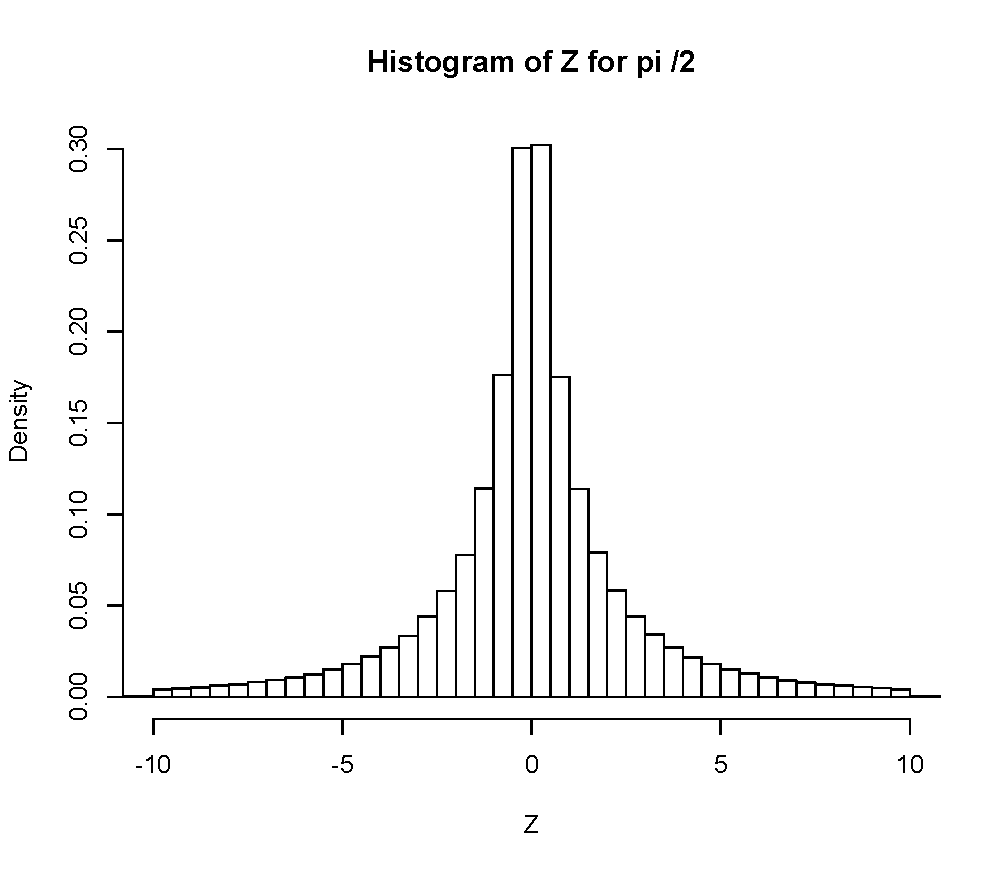
\includegraphics[width=0.8\textwidth]{pi2plot.pdf}
\caption[]{ 
 Distribution of zeta values at $\phi = \pi/2$.
  }
\vspace{1mm}
\label{pi2}
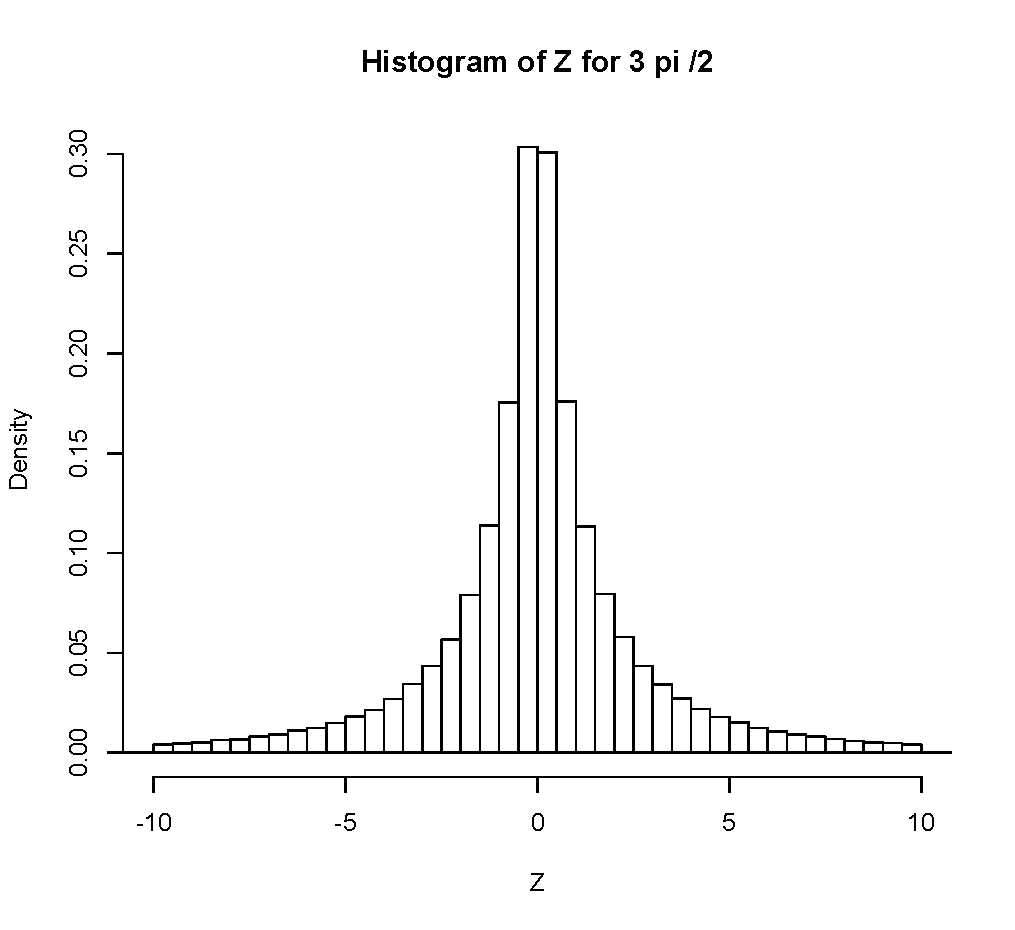
\includegraphics[width=0.8\textwidth]{3pi2plot.pdf}
\caption[]{ 
 Distribution of zeta values at $\phi = 3\pi/2$.
  }
\vspace{1mm}
\label{3pi2}
\end{figure*}

\begin{figure}
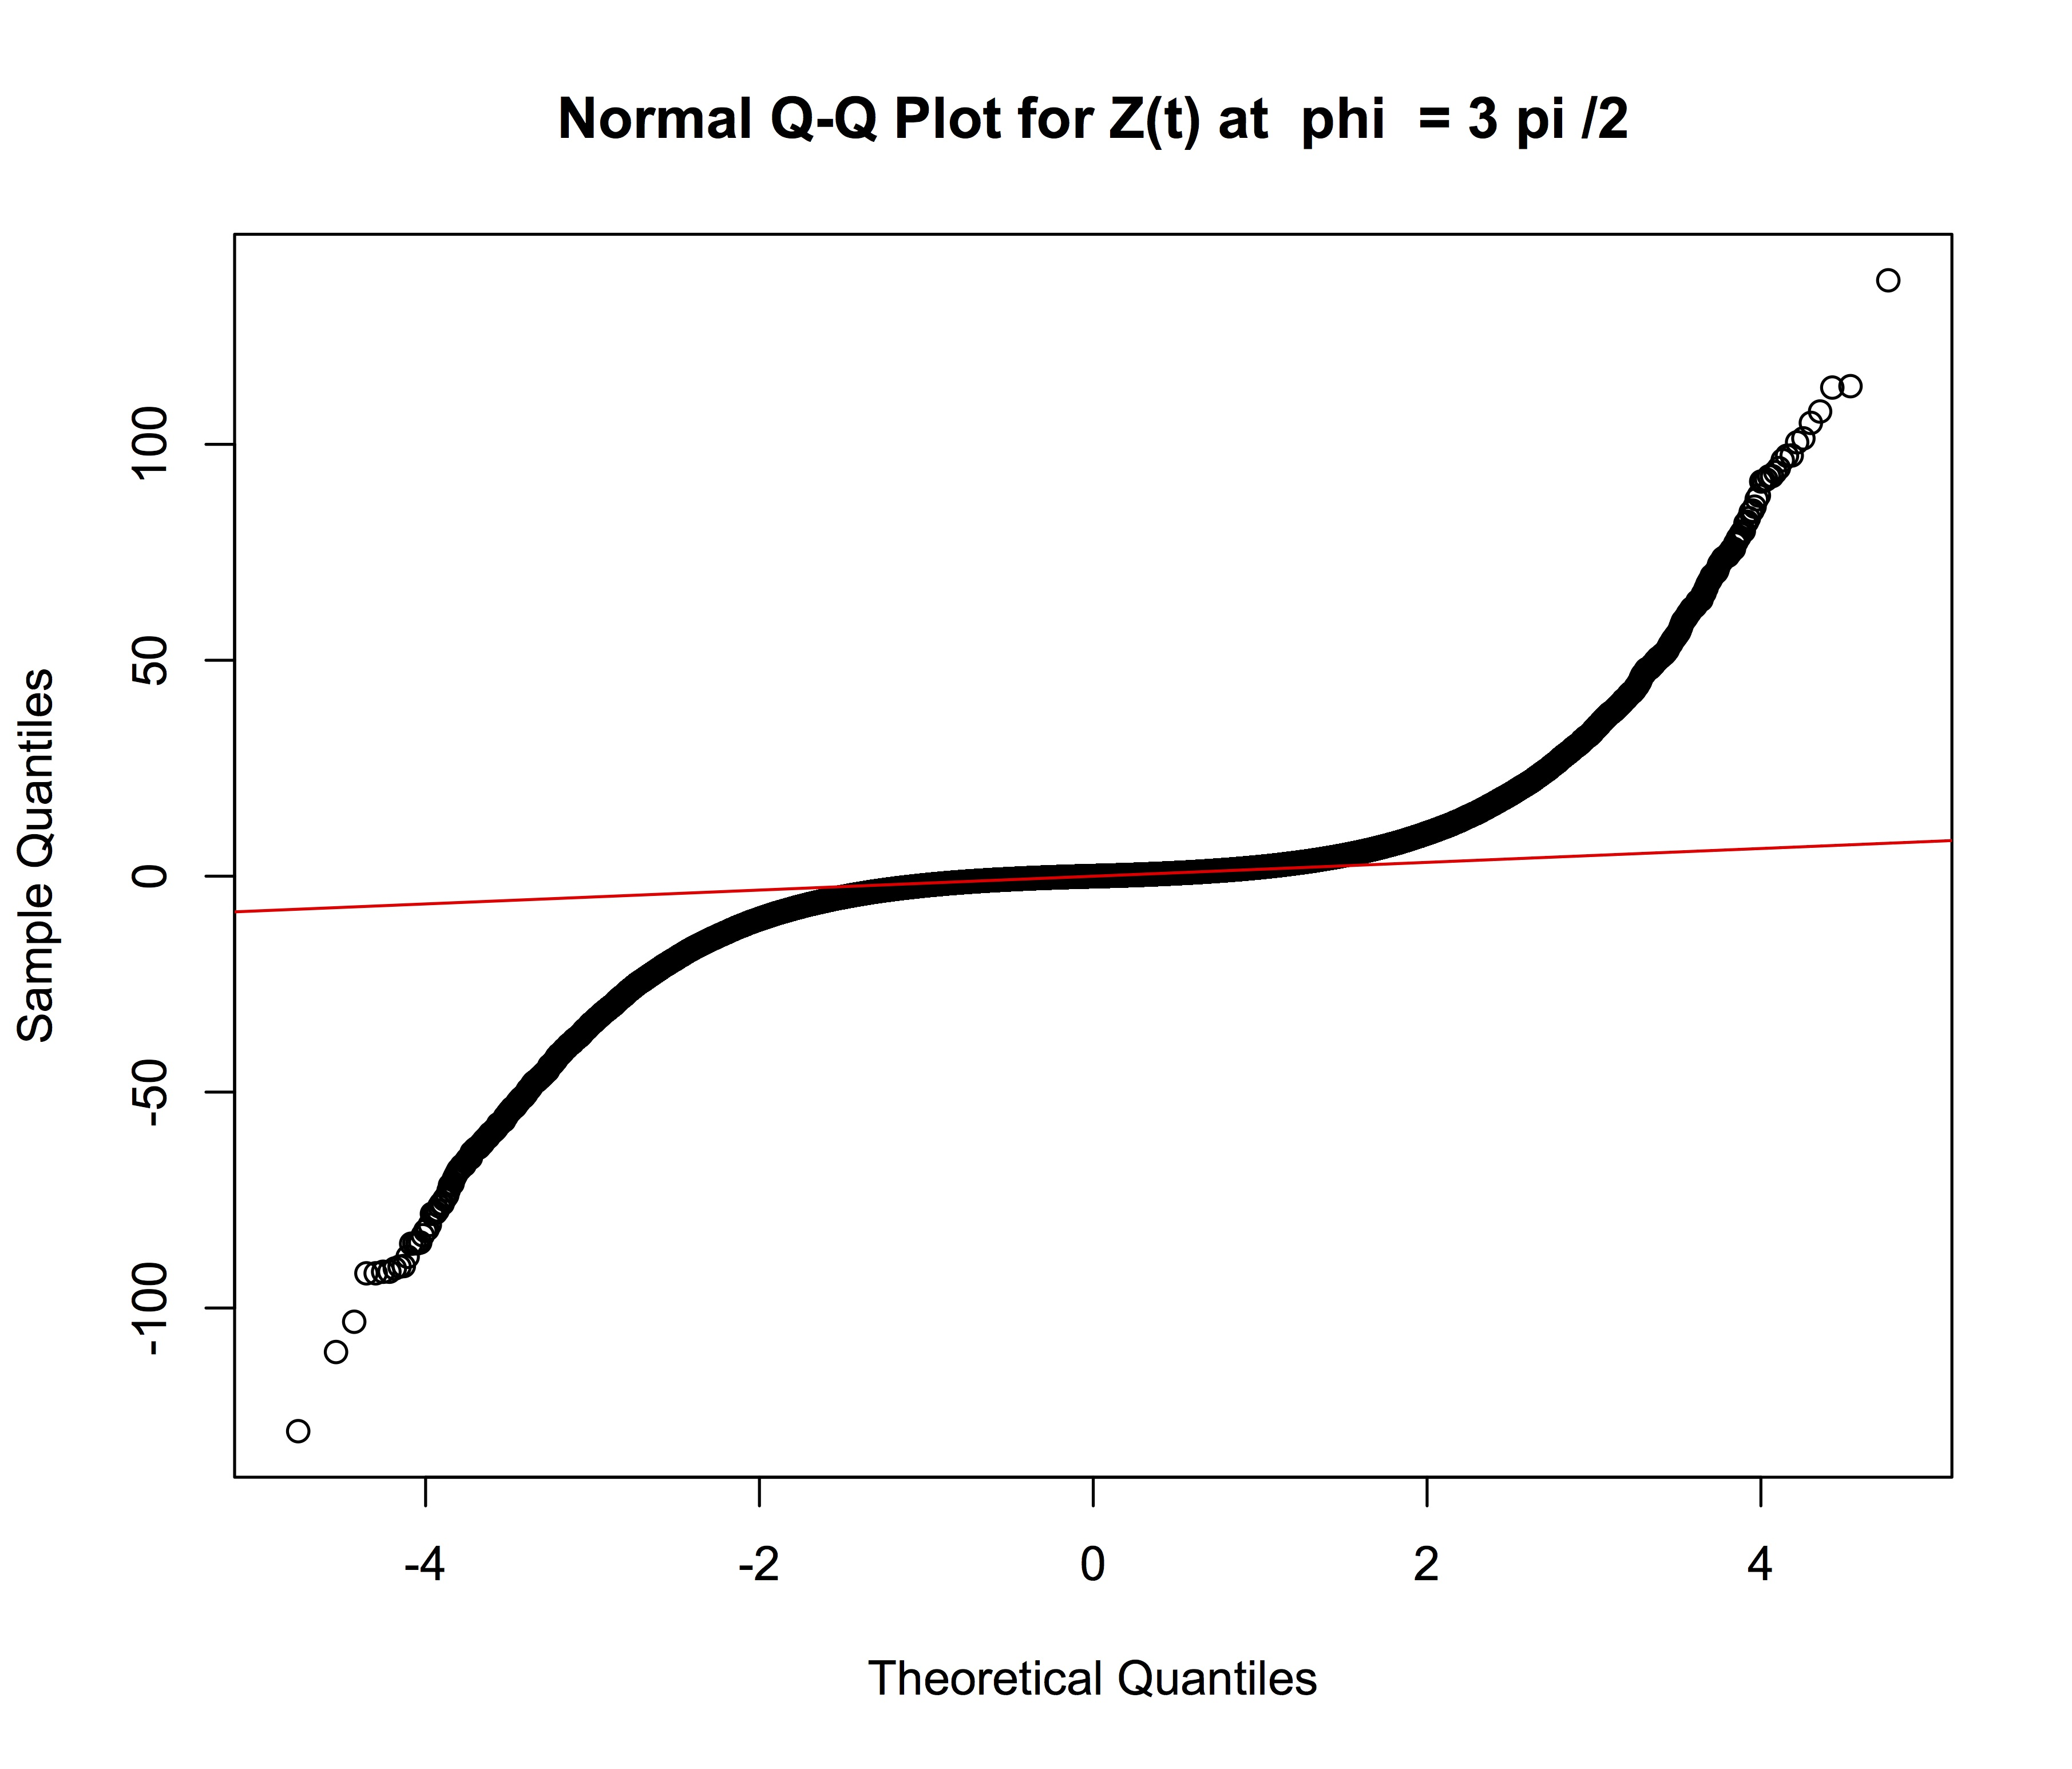
\includegraphics[width=0.8\textwidth]{qqplot.jpg}
\caption[]{ 
 QQ plot of zeta values at $\phi = 3\pi/2$.
  }
\vspace{1mm}
\label{qqplot}
\end{figure}

\subsection{\label{kurtosis}Skewness and kurtosis}
Table~\ref{tab:kurtosis4} shows the skewness and kurtosis for  $Z(t)$  when $\phi$ values are multiples of $\pi/4$.  
Table~\ref{tab:kurtosis6} shows the skewness and kurtosis for  $Z(t)$  when $\phi$ values are multiples of $\pi/6$.  
The tables show that the distributions are symmetric for reflections around Gram points ($\phi = 0$ and $\phi= \pi$) and anti-symmetric for reflections around the mid-points of Gram intervals ($\phi = \pi/2$ and $\phi = 3\pi/2$). The large values of  kurtosis show that the distributions tend to have heavy tails, or outliers. The distributions  also have large skew, except for $\phi = \pi/2$ and $\phi = 3\pi/2$, where the distributions are symmetric. There seems to be a small systematic deviation for the skewness, maybe due to the fact that we take the Gram interval to be constant over $34$ sub-intervals of the sample space.

\subsection{\label{histograms}Histograms}
Ref.~\cite{Shanker 2018}  presented figures for the histograms at even and odd Gram points, which are the histograms for $\phi=0$ and $\phi=\pi$ respectively. Fig.~\ref{pi2} shows 
the histogram for $\phi = \pi/2$. Our conjectures predict that the histogram has the same distribution as the distribution for $\phi = 3\pi/2$. Further, the conjectures predict that for this $\phi$ the distribution will be symmetric (this is required if both  Equations  \ref{eq:antisym} and \ref{eq:sym} are to be satisfied). Fig.~\ref{3pi2} shows 
the histogram for $\phi = 3\pi/2$. The predictions are validated. While  the histograms are symmetric, the distribution is not normal. This can be seen from the QQ plot, which is exhibited in Fig.~\ref{qqplot} for $\phi = 3\pi/2$. The plot shows that the distribution has a fatter tail than would be expected for a normal distribution.

\section{\label{conclusions}Conclusions}

In this work we defined phi points on the critical axis, in analogy with Gram points. We used this definition to extend the results of Ref.~\cite{Shanker 2018}.  Conjecture 1 of that reference stated an anti-symmetry property of the distribution of $Z$ values at even and odd Gram points. In this work we formulated three new symmetry related conjectures. The conjectures are the mean value condition  Equation \ref{eq:mean}, the anti-symmetry condition  Equation \ref{eq:antisym} and the symmetry condition  Equation \ref{eq:sym}. These conjectures are a generalization of Conjecture 1 in 
Ref.~\cite{Shanker 2018} to phi points. Theoretical study of the relations presented here needs to be done.


\begin{thebibliography} {}

\bibitem{Shanker 2018} O. Shanker, 
``Good to Bad Gram Point Ratio For Riemann Zeta Function",
{\it Experimental Mathematics} {\bf doi:10.1080/10586458.2018.1492474}(2018)



\bibitem {Riemann(1858)} B. Riemann, ``\"{U}ber die Anzahl der Primzahlen uter
Einer Gegebenen Gr\"{o}be,'' {\it Montasb. der Berliner Akad.}, (1858),
671-680

\bibitem {Riemann 1892} B. Riemann, ``Gesammelte Werke'', Teubner, Leipzig, (1892)

\bibitem {Titchmarsh 1986} E. Titchmarsh, ``The Theory of the Riemann Zeta
Function,'' Oxford University Press, Second Edition, (1986)

\bibitem {Edwards(1974)} H. M. Edwards, ``Riemann's Zeta Function,''
Academic Press,  (1974)

\bibitem{Gram 1903} J. P. Gram, 
``Sur les Zeros de la Fonction  $\zeta ( s )$  de Riemann",
{\it Acta Math.} {\bf27}(1903), 289-304

\bibitem{Titchmarsh 1934} E. C. Titchmarsh,
``On van der Corput's method and the zeta-function of Riemann (IV)",
{\it Quart. J. Math. Oxford Ser.} {\bf5}(1934), 98-105

\bibitem{hiary 2010} G. A. Hiary,
``An amortized-complexity method to compute the Riemann zeta function", 
{\it Mathematics of Computation} {\bf80}(2011), 1785-1796

\bibitem{Odlyzko 1992}  A. Odlyzko,
``The $10^{20}$-th Zero of the Riemann Zeta
Function and 175 Million of its Neighbors", report,
\url{http://www.dtc.umn.edu/~odlyzko/unpublished/zeta.10to20.1992.pdf}, (1992)

\bibitem{hiary} G. A. Hiary,
``Fast methods to compute the Riemann zeta function",
{\it Annals of Mathematics} {\bf63}(1987), 891-946

\bibitem{gourdon} Xavier Gourdon,
``The $10^{13}$ first zeros of the Riemann Zeta function,
and zeros computation at very large height", report,
\url{http://numbers.computation.free.fr/Constants/Miscellaneous/zetazeros1e13-1e24.pdf}, (2004)


\end{thebibliography} 

\end{document} 
